\chapter{Uncertainty in atomic force predictions}
\label{chapter3}



Optimal ensembling averaging of neural networks: \cite{optimal_ensemble_averaging_naftaly}\\
Ensemble deep learning: a review: \cite{ensemble_deep_learning_review_ganaie}\\
Addressing uncertainty in atomistic machine learning: \cite{uncertainty_atomistic_ml_peterson}\\
Quality of uncertainty estimates from neural network potential ensembles: \cite{uncertainty_of_nnp_ensembles_kahle}\\
Uncertainty quantification in molecular simulations with dropout neural network potentials: \cite{uncertainty_quantification_dropout_wen}\\
Explainable uncertainty quantifications for deep learning-based molecular property prediction: \cite{uncertainty_quantification_yang}\\
Evaluating scalable uncertainty estimation methods for deep learning-based molecular property prediction : \cite{scalable_uncertainty_scalia}\\
Simple and scalable predictive uncertainty estimation using deep ensembles: \cite{scalable_uncertainty_lakshminarayanan}\\



\section{Potential solution}
\label{sec:uncertainty_potential_solution}
Looking for some atomistic value to use as a metric for molecular energy prediction, without actually knowing the ground truth to compare that prediction to. 

Atomic energies were a wash, there seems to be no way to reduce the predictive uncertainty of these values without making the "desired" prediction of molecular energy a higher-error prediction. 

We need something that is supported by \textit{ab initio} theory, which our networks can predict in a streamlined way in order to estimate the uncertainty of predictions at an atomistic level. There is only one quantity which exists for every atom: forces. (Could talk about dipoles here, and possibly mention how dipoles are sometimes non-existent, but the forces acting upon atoms usually aren't -- at most they are such a small value that they're considered zero -- but we don't really explore global equilibrium with MD so this shouldn't be an issue).

\subsection{Forces}
\label{subsec:forces}

\begin{figure}[H]
    \centering
    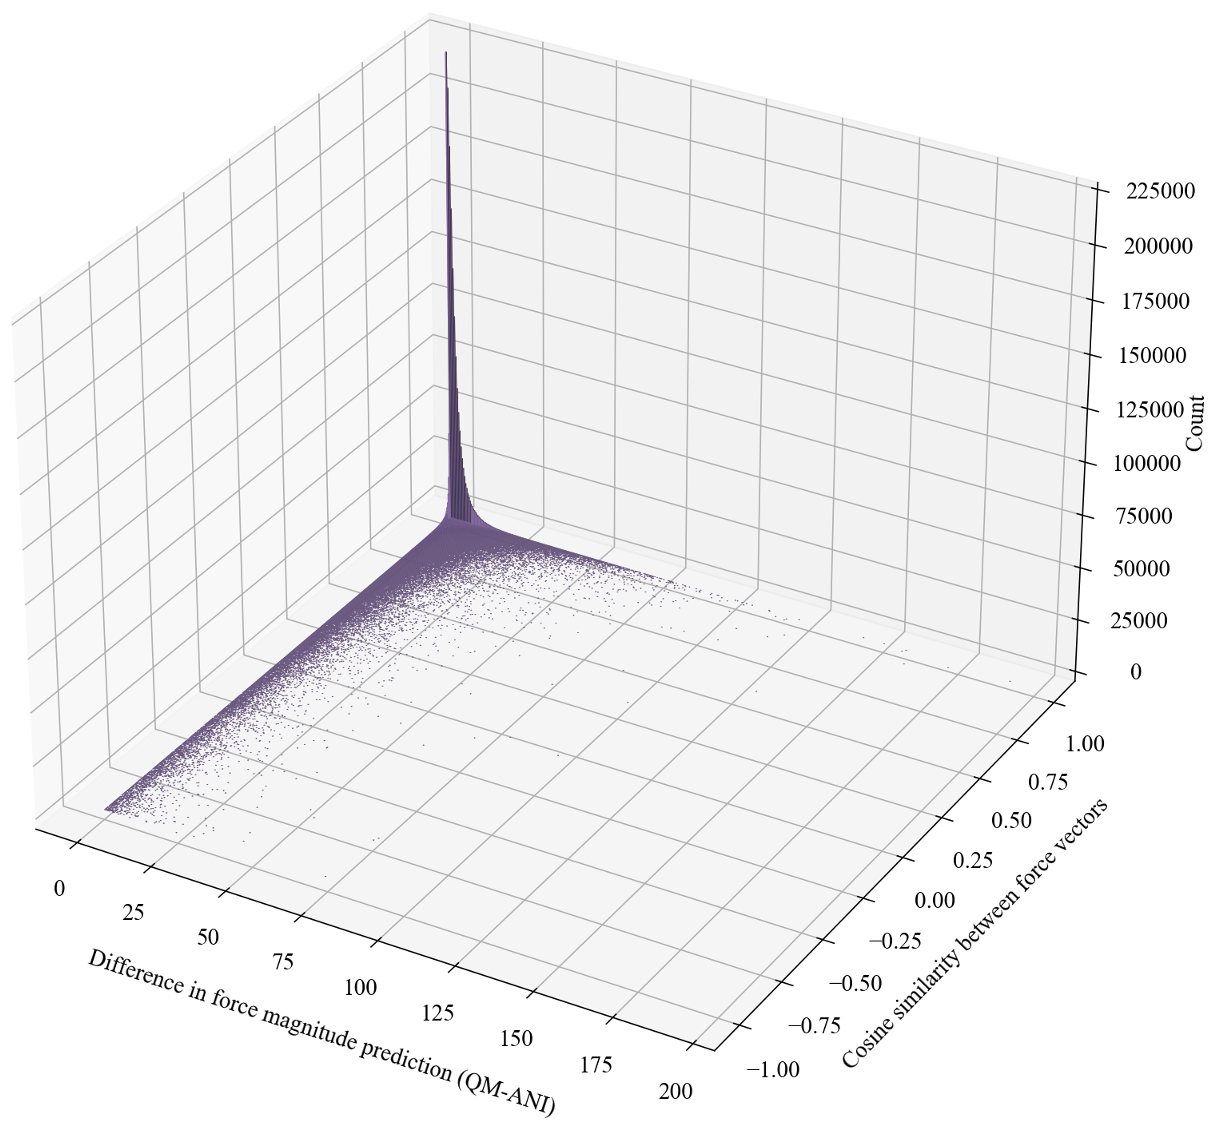
\includegraphics[width=1\linewidth]{Images/2xr_forces/2xr_comp6v1_force-cosine_sim-bar3d.png}
    \caption[Per-model cosine similarity measure of predicted atomic force vectors]{
    Cosine similarity between ANI predicted forces (per-model) versus the DFT reference forces on the COMP6v1 benchmark dataset.
    }
    \label{fig:2xr_comp6v1-forces-cos_sim}
\end{figure}

\subsection{Force magnitudes}
\label{subsec:force_magnitudes}

\begin{figure}[H]
    \centering
    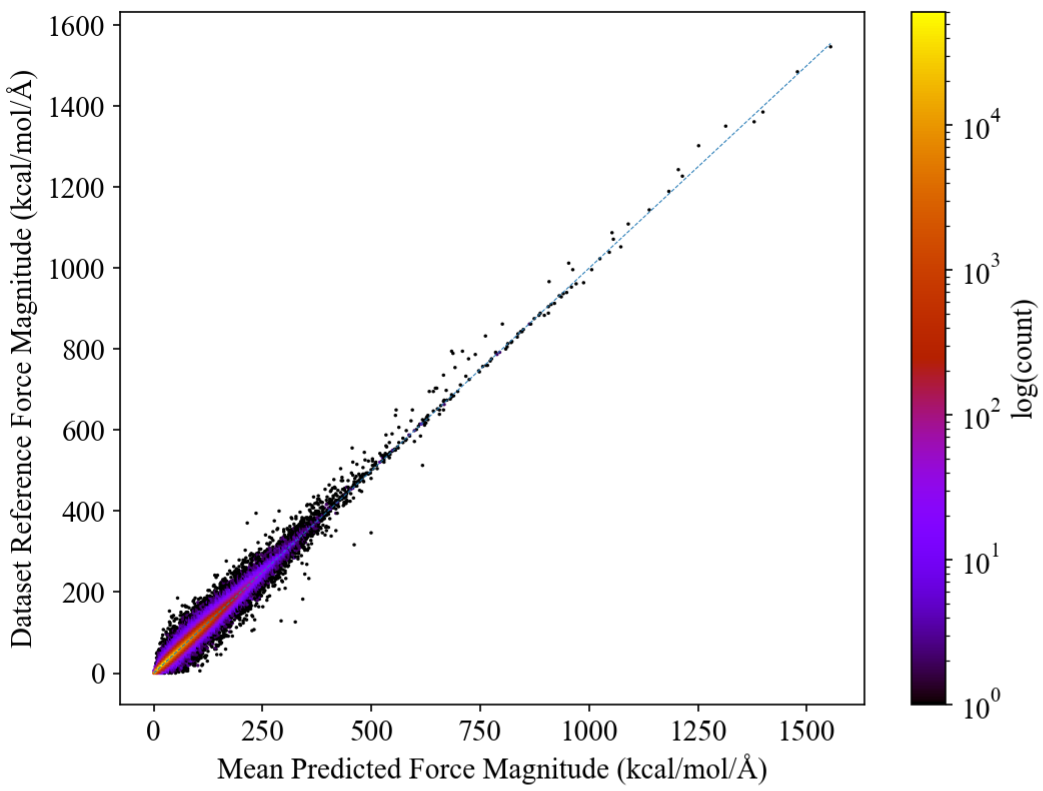
\includegraphics[width=1\linewidth]{Images/2xr_forces/2xr_comp6v1_force-dft-vs-mean_ani.png}
    \caption[Mean predicted atomic force magnitude vs DFT reference]{Predicted force magnitudes vs DFT reference force magnitudes on the COMP6v1 benchmark dataset.}
    \label{fig:2xr_comp6v1-forces-ani_vs_ref}
\end{figure}

\section{Analyzing the Uncertainty of Force Predictions}
\label{sec:analyzing_force_uncertainty}

\begin{figure}[H]
    \centering
    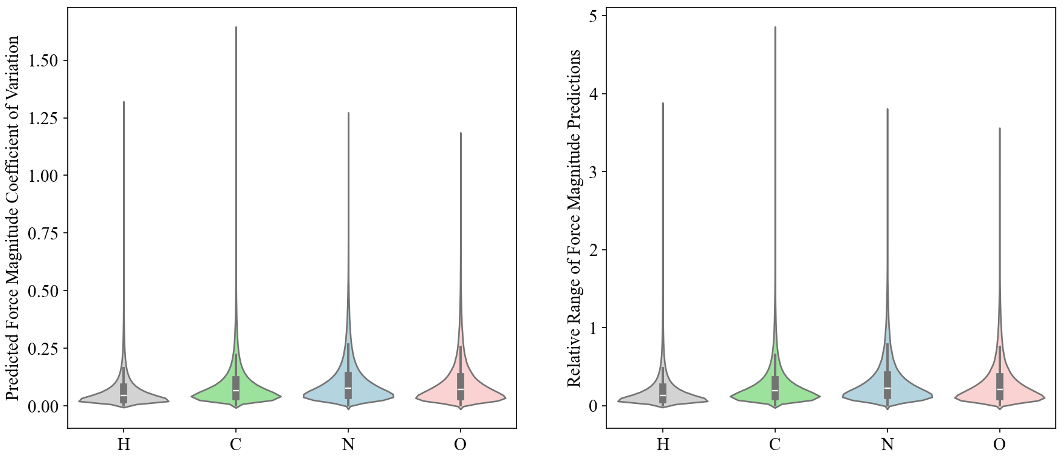
\includegraphics[width=1\linewidth]{Images/2xr_forces/2xr_comp6v1_force-uncertainty_violin.png}
    \caption[Uncertainty in force magnitude predictions: violin distribution]{Violin distribution of force magnitude uncertainty measures, computed for ANI-2xr predictions on the COMP6v1 benchmark dataset.}
    \label{fig:2xr_comp6v1-force_uncertainty-violin}
\end{figure}

\begin{figure}[!hp]
    \centering
    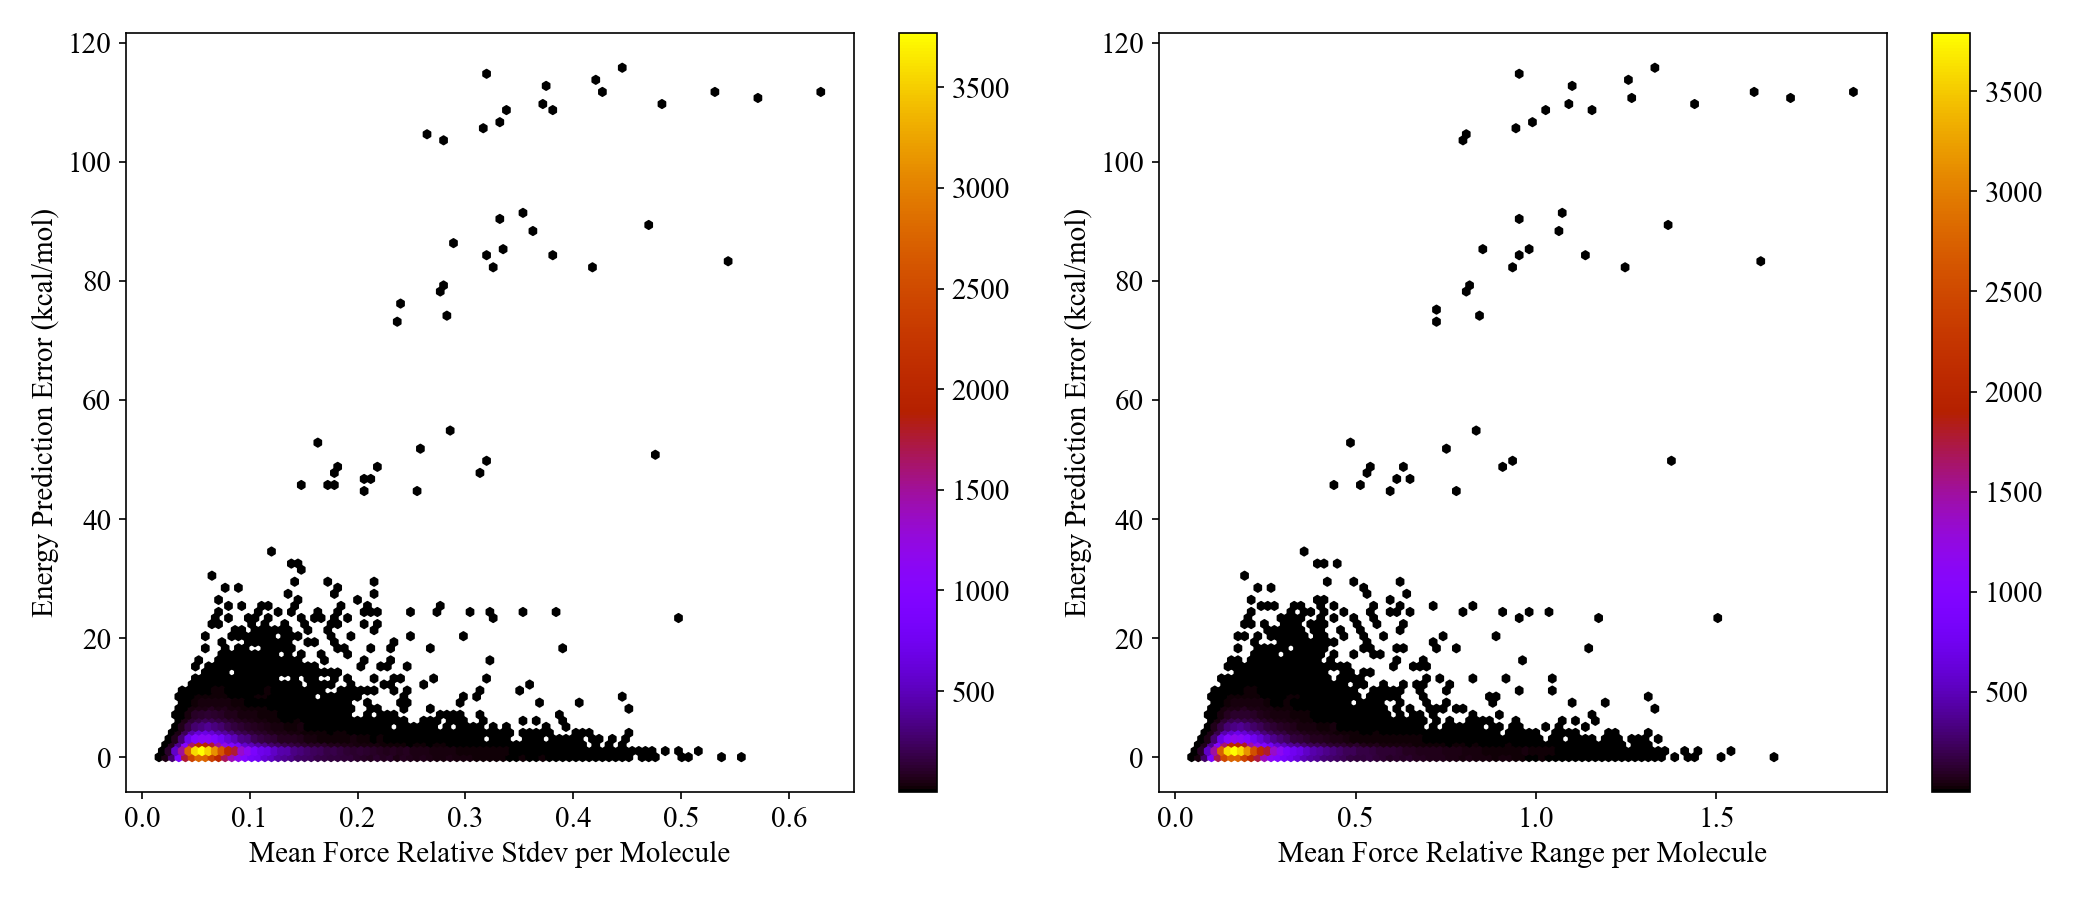
\includegraphics[width=1\linewidth]{Images/2xr_forces/2xr_comp6v1_force-mean-uncertainty-vs-energy.png}
    \caption[Average force uncertainty measures per-molecule versus energy error (COMP6v1)]{Averaged uncertainty measures per-molecule on the ANI-2xr predicted forces versus the energy error for the COMP6v1 benchmark dataset.}
    \label{fig:2xr_comp6v1-mean_force_uncertainty_hexbin}
\end{figure}

\begin{figure}[!hp]
    \centering
    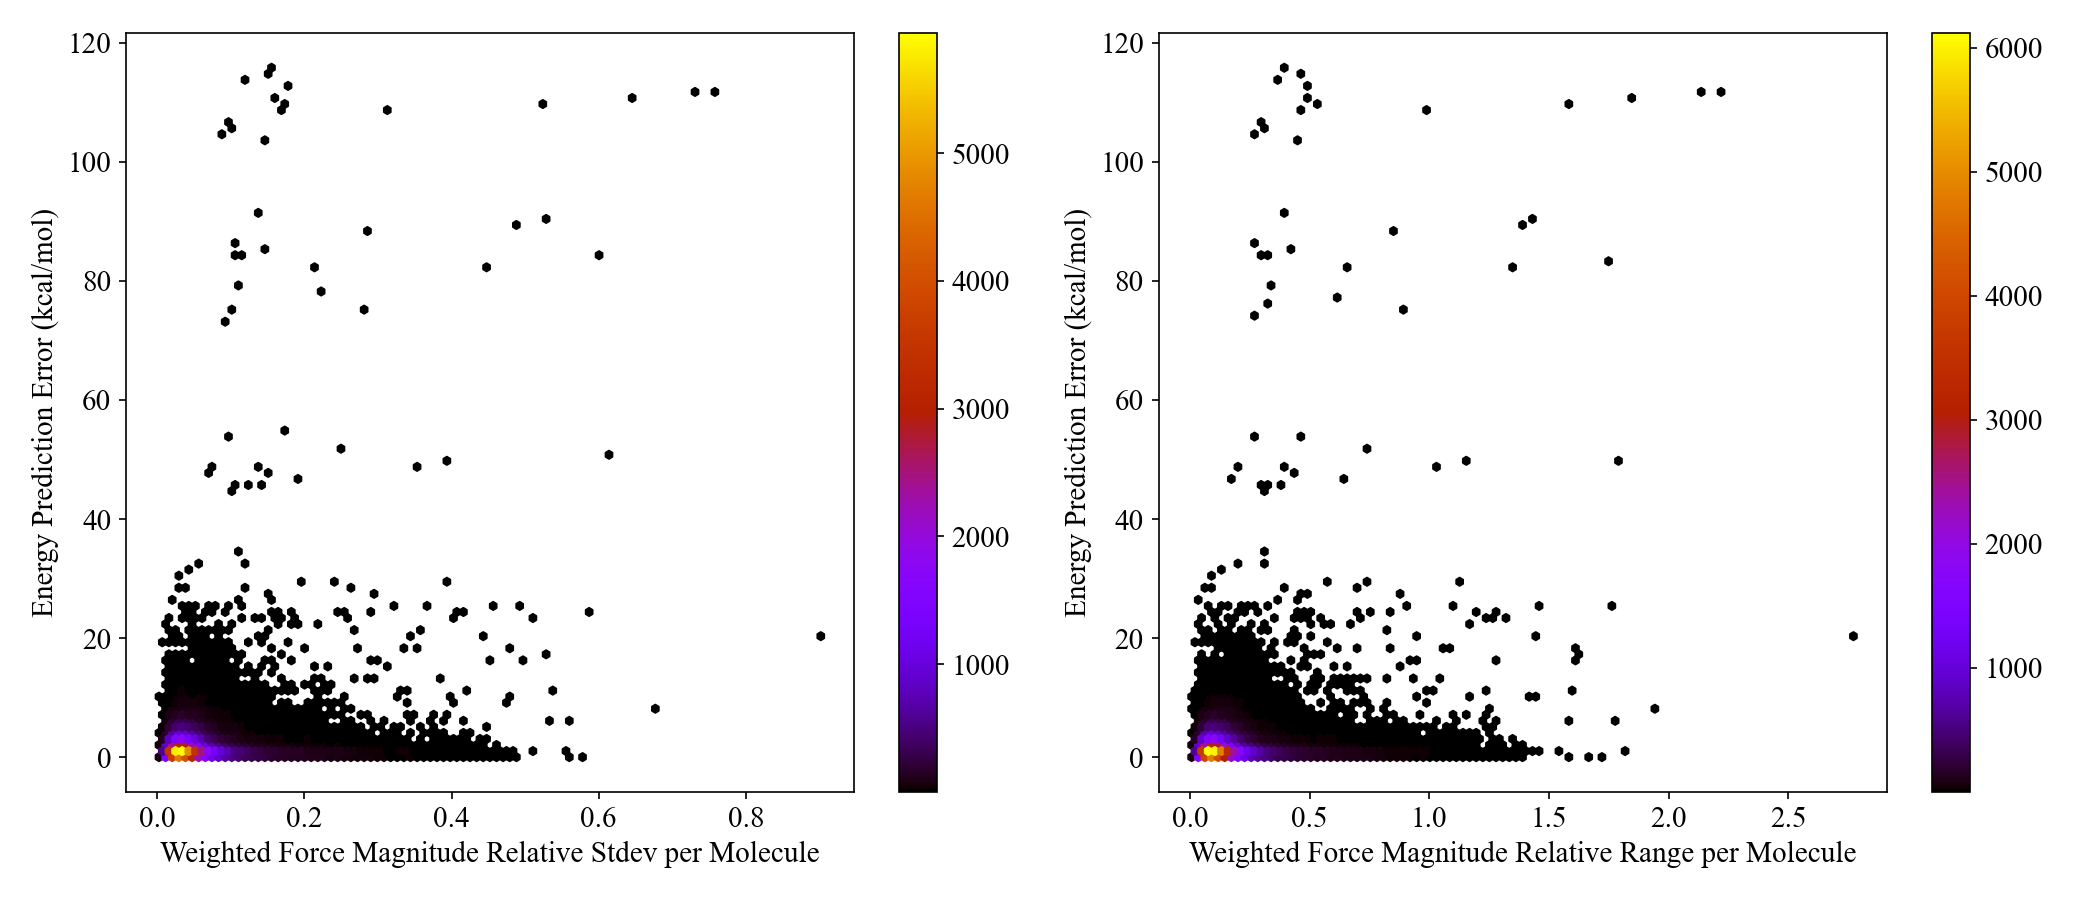
\includegraphics[width=1\linewidth]{Images/2xr_forces/2xr_comp6v1_force-weighted-uncertainty-vs-energy.png}
    \caption[Force uncertainty weighted by outliers versus energy error (COMP6v1)]{Outlier-weighted uncertainty measures for ANI-2xr predicted force magnitudes versus the energy error on the COMP6v1 benchmark dataset.}
    \label{fig:2xr_comp6v1-forces-weighed_uncertainty}
\end{figure}

\begin{figure}[!hp]
    \centering
    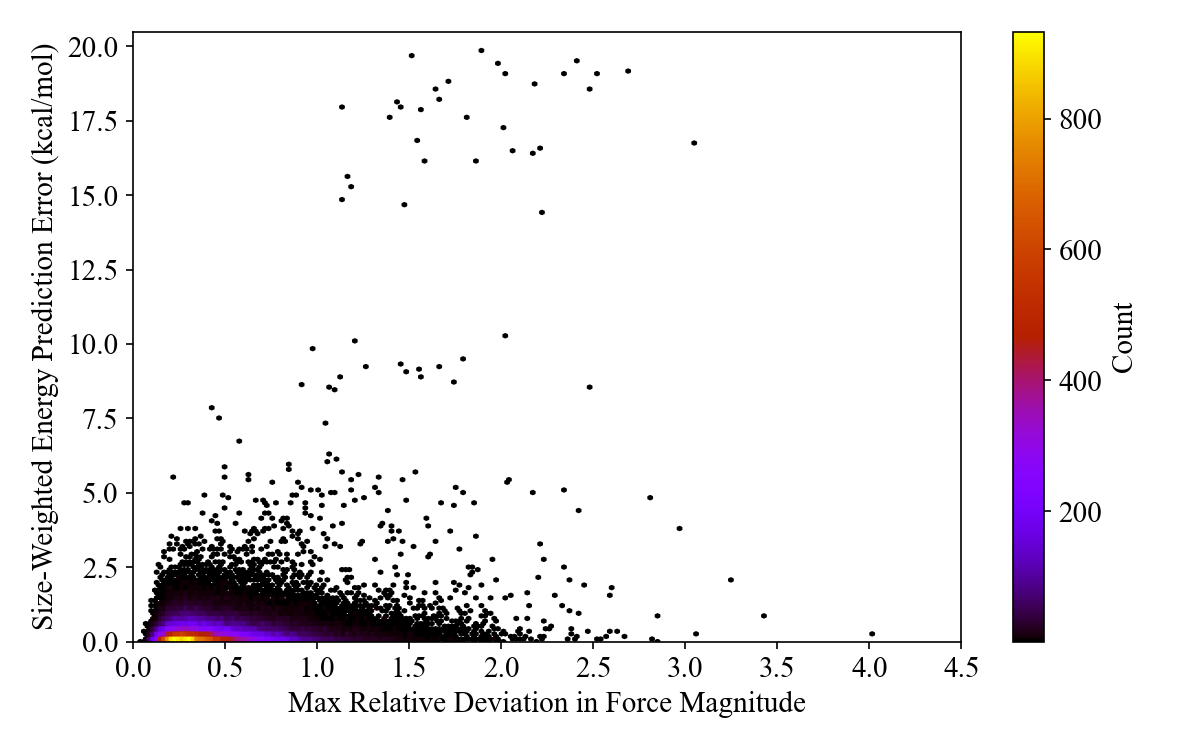
\includegraphics[width=1\linewidth]{Images/2xr_forces/2xr_comp6v1_force-highest-force_deviation-vs-energy.png}
    \caption[Maximum deviation in force magnitude prediction versus energy error (COMP6v1)]{Maximum deviation in force magnitude prediction by ANI-2xr versus energy error on the COMP6v1 benchmark dataset.}
    \label{fig:2xr_comp6v1-forces-highest_deviation}
\end{figure}


\subsection{Atom isolator}
\label{subsec:atom_isolator}
Capping atoms

Molecular representations in AI-driven drug discovery (a review): \cite{mol_reps_in_AI_drug_discovery_david}\\
SMILES and SMARTS papers: \cite{SMILES_pair_encoding_li, mol_patterns_SMARTS_schmidt, automated_fragment_gen_smiles_bilsland}\\
Protein fragmentation with neural networks: \cite{protein_ff_fragmentation_nn_wang}\\
Escaping atom types in force fields using direct chemical perception: \cite{direct_chem_perception_mobley} \\

\subsection{Drawback: configurational sampling}
\label{subsec:drawback_config_sampling}

GDB-13: \cite{gdb-13}
GDB-17: \cite{gdb-17}
ChEMBL: \cite{ChEMBL_gaulton}

Another novel approach to producing new configurations of atoms is explored in \hyperlink{configurational_sampling}{Chapter 5}.

\section{Outlook}